%!TEX root = ../main.tex
\chapter{異なる学習率を用いた予備実験の結果}

\ref{sec:lr}章にて行った予備実験にて,異なる学習率を用いた場合の結果のグラフを以下に示す.

まず,RBMの学習時におけるエポック数とクロスエントロピーの関係について示した後,出力層の学習におけるエポック数と誤差の関係について示す.

\begin{figure}[]
\begin{center}
   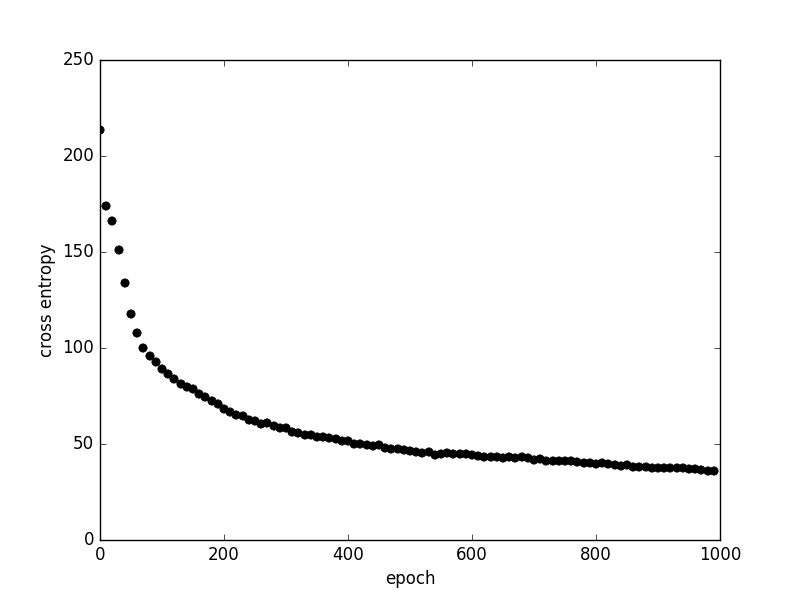
\includegraphics[scale=0.8]{./koki/ent001.png} \\
   \caption{RBMの学習の様子(学習率0.01)}
\end{center}
\end{figure}

\begin{figure}[]
\begin{center}
   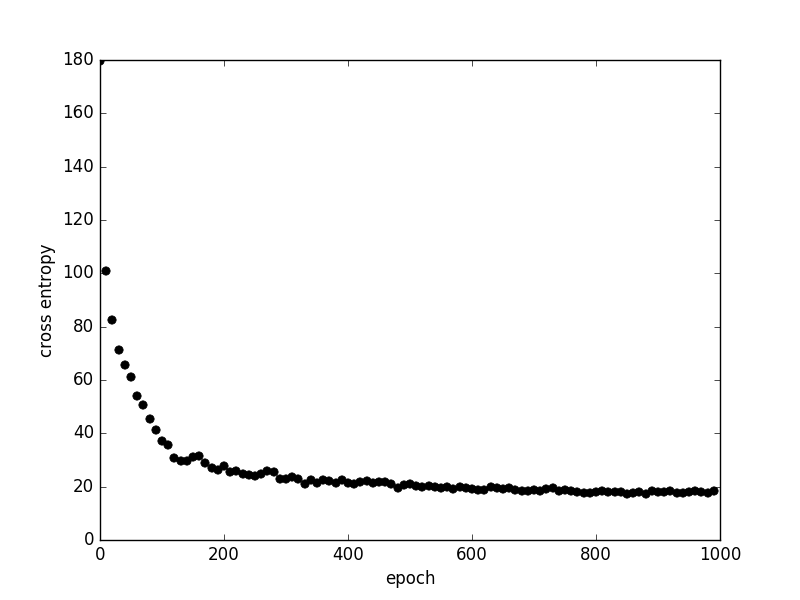
\includegraphics[scale=0.8]{./koki/ent005.png} \\
   \caption{RBMの学習の様子(学習率0.05)}
\end{center}
\end{figure}

\begin{figure}[]
\begin{center}
   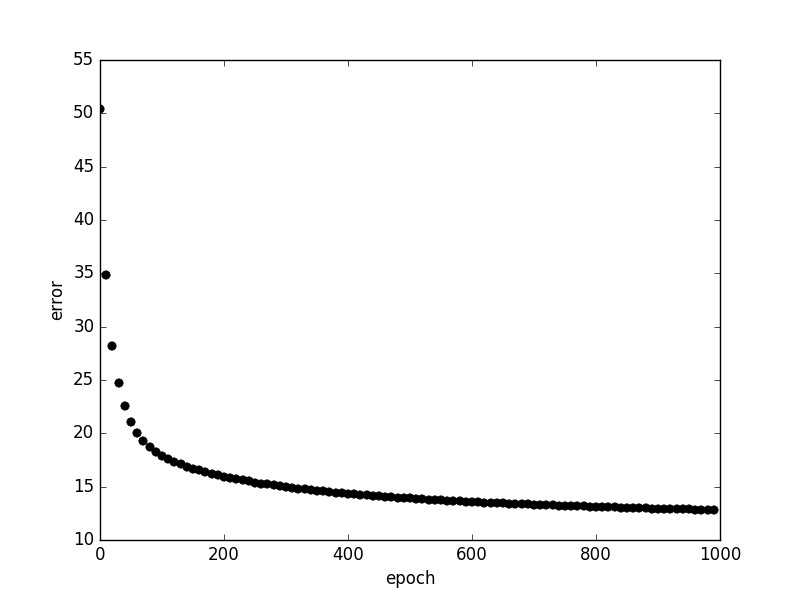
\includegraphics[scale=0.8]{./koki/err001.png} \\
   \caption{出力層の学習の様子(学習率0.01)}
\end{center}
\end{figure}

\begin{figure}[]
\begin{center}
   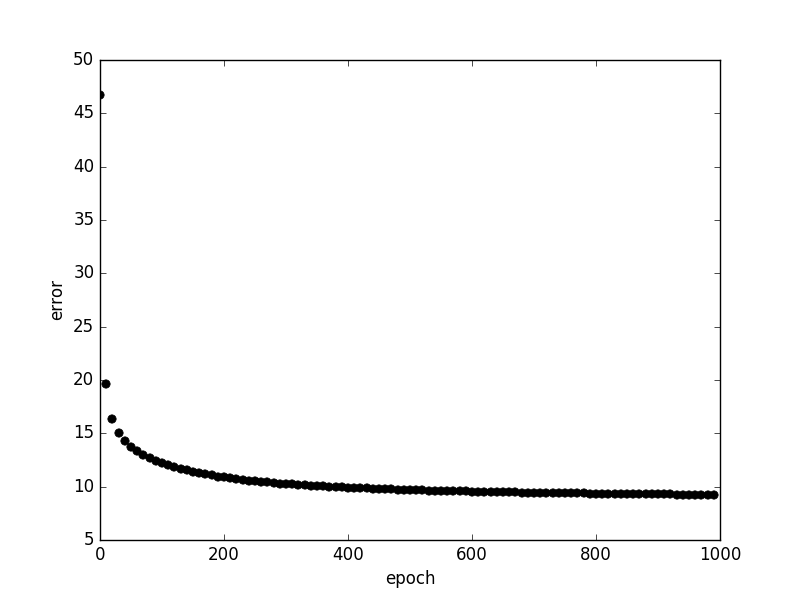
\includegraphics[scale=0.8]{./koki/err005.png} \\
   \caption{出力層の学習の様子(学習率0.05)}
\end{center}
\end{figure}